\chapter{Literature Review}
\label{chap:lr}
\chaptermark{Second Chapter Heading}

%\Blindtext[2]

\section{RNN Encoder-decoder}

\cite{B}

\begin{align}
\label{prob-trans}
\ p(y) = \prod_{t=1}^{T} p(y_t | \{y_1, \dots, y_{t-1}\}, c),
\end{align}
where $y = (y_1, \dots, y_{T_{y}})$. The reference to equation (\ref{prob-trans}) is clickable. 

\section{Attention}
Introduction of recurrent neural network encoder-decoder architecture has revolutionised machine translation. However, they have suffered from one critical flaw: deterioration of performance with increasing of input sentence length\cite{C}. Authors have evaluated Encoder–Decoder against baseline phrase-based statistical model Moses \cite{D} using BLEU score \cite{E}. The results have demonstrated clear degradation of performance on longer sentences. The authors hypothesize that this issue is caused by scarcity of fixed-length vector's capacity to encode a long sentence with complicated structure and meaning.

This bottleneck was addressed in \cite{A}. The authors have introduced an approach which encodes the input sequence into a sequence of vectors, annotations. They are used in decider choose parts of the sentence it should pay attention to. This approach relieves the encoder from burden of capturing information about whole source sentence.

The attention mechanism provides new formula for conditional probability of getting next word of translation $y_i$ given previously predicted words:
\begin{align}
\label{att-prob}
\ p(y_i| y_1, \dots, y_{i-1}, x) = g(y_{i-1}, s_i, c_i),
\end{align}
where $s_i$ is an RNN hidden state for time i:
\begin{align}
\ s_i = f(s_{i-1}, y_{i-1}, c_i).
\end{align}

\begin{figure}[H]
\centering
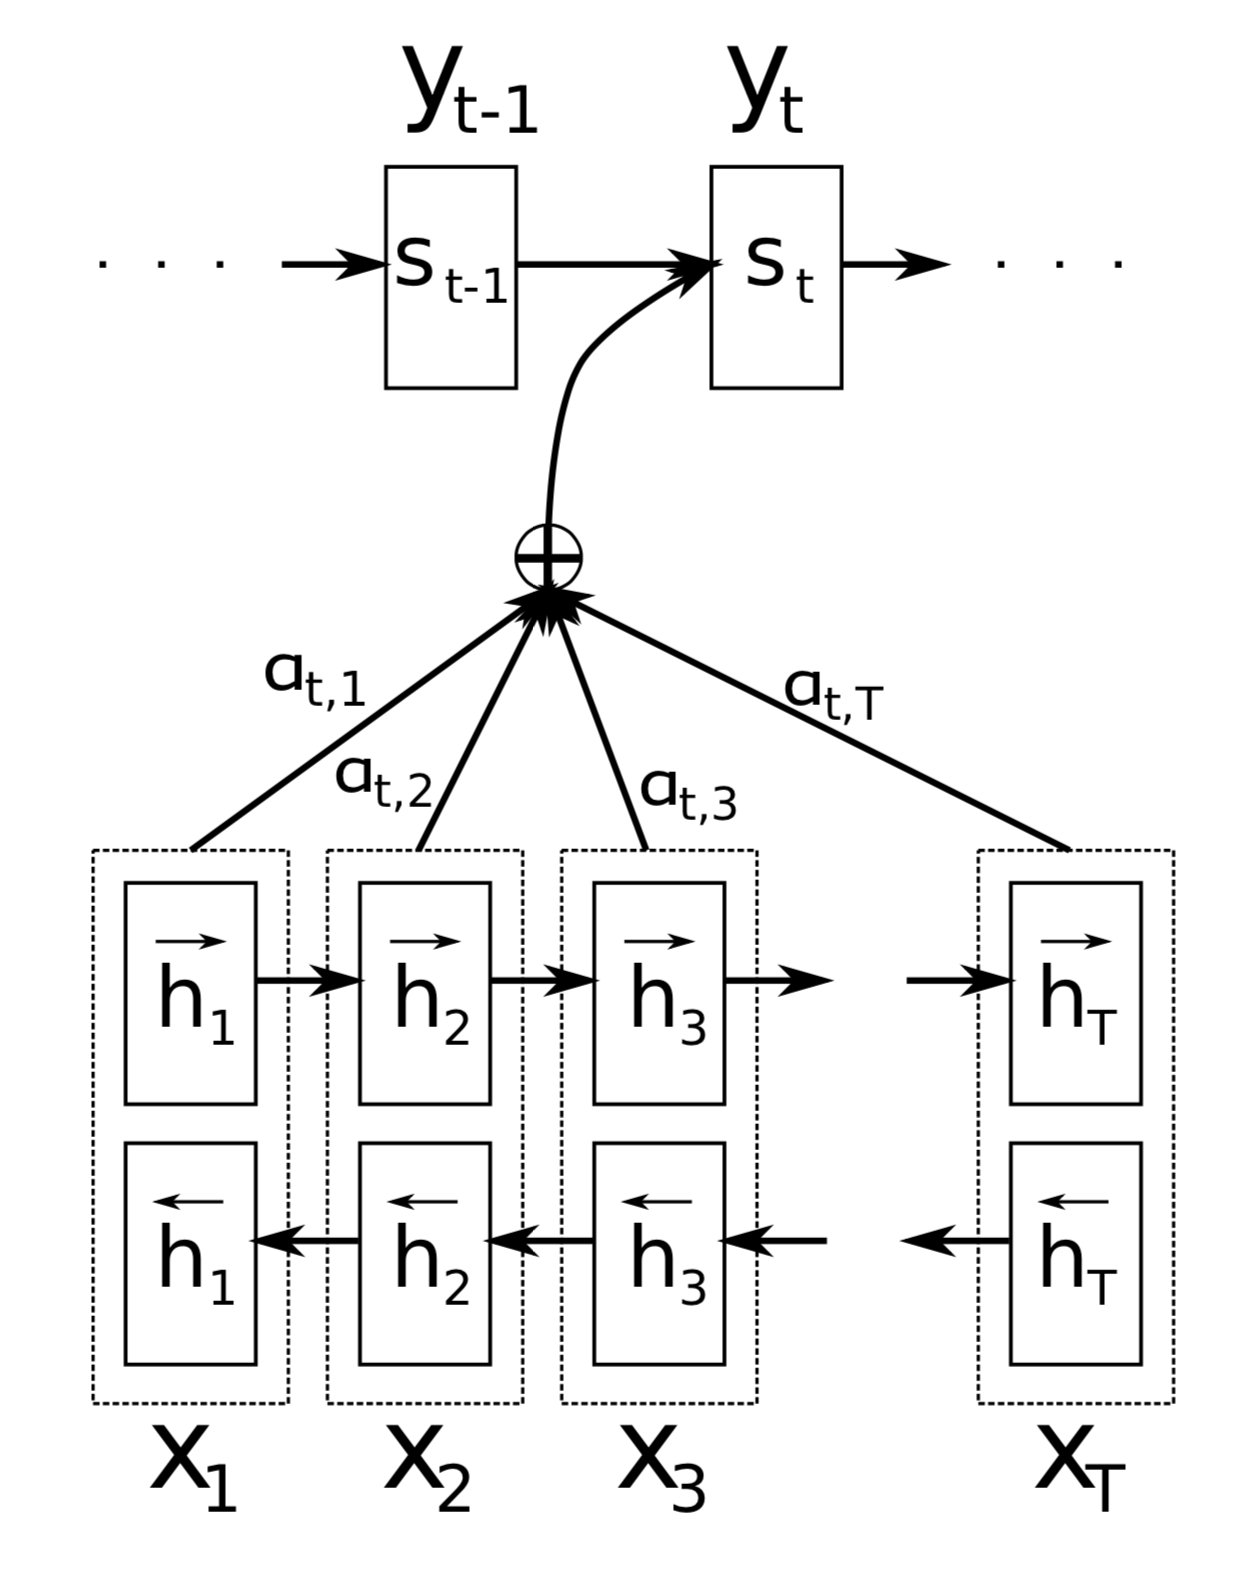
\includegraphics[width=0.3\textwidth]{figs/attention.png}
\caption[Attention model illustration]{Attention model illustration.}
\label{att-ill}
\end{figure}

The Figure \ref{att-ill} illustrates the proposed model generating the $t$th target word $y_t$ given a source sentence $(x_1,x_2,...,x_T )$.

The encoder is used to calculate sequence annotations and consists of two RNNs: backward and forward. This is done to capture both preceding and following words. Reading the sequence from both directions results in two sets of RNNs' hidden states: forward - $(\overrightarrow{h_1}, \dots, \overrightarrow{h_{T_x}})$; and backward - $(\overleftarrow{h_1}, \dots, \overleftarrow{h_{T_x}})$. Each pair of corresponding vectors is concatenated to form a final set of sequence annotations: $h_j = [\overrightarrow{h_j}; \overleftarrow{h_j}]^T$.

Each context $c_i$ is computed as a weighted sum of sequence of annotations $(h_1, \dots, h_{T_{x}})$:

\begin{align}
\label{cont-vec}
\ c_i = \sum_{j=1}^{T_x} \alpha_{ij}h_j.
\end{align}

The weight $\alpha_{ij}$ of each annotation $h_j$ is computed by

\begin{align}
\label{ann-weight}
\ \alpha_{ij} = \frac{exp(e_{ij})}{\sum_{k=1}^{T_x}exp(e_{ik})},
\end{align}
where
\begin{align}
\ c_{ij} = a(s_{i-1}, h_j).
\end{align}
is an alignment model that evaluates how well the inputs around position $j$ and the $i$th output match. It is parametrized as a feedforward neural network. Each weight can be seen as a probability that the target word $y_i$ is aligned to a source word $x_j$, and it reflects the importance of annotation with respect to a previous hidden state in generating next output word $y_i$ and deciding the next state. This implements a mechanism of attention in decoder, which lets it decide the most important part of source sentence for each step of translation. 

%\Blindtext[1]
